This \chap\ presents techniques added to Smokeview~\cite{Smokeview_Tech_Guide} applicable
for visualizing WUI (wildland urban interface) and wild fire scenarios.  Two techniques
involve 1) visualizing changing terrain using satellite images with modeling results
overlayed and 2) making use of geometric objects for representing modeling elements
such as trees or building structures. These two techniques use data generated by fire
models such as FDS~\cite{FDS_Tech_Guide}.
A third technique involves visualizing experimentally derived data rather than modeling
data.  Wind sensor data is visualized using flow vectors along with visual indicators
of data uncertainty. Smokeview images are displayed in the following figures to
illustrate these techniques.

Figure \ref{figlevelset} presents contours of a level set computation.
The level set contours are drawn on a sloped terrain. These level set
contours represent a fire line. A fire line is used with wildland fire
simulations as an efficient method for visualizing the motion of a fire
across the simulation. A fire line in the context of Smokeview is just a
special case of a temperature slice contour.  The thin red line represents
the location where burning is currently taking place.  The grey region
represents where burning has occurred and the green region represents
where burning has not occurred. Level sets are used to quickly (relative
to a complete computational fluid dynamic calculation ) model fire spread
and fire line locations. In this particular case, images are drawn at
\SI{30}{s}, \SI{60}{s}, \SI{90}{s} and \SI{120}{s}. The test verifies
that the level set slices follow the sloped terrain. 
%Figure \ref{figterrain2}
%and \ref{figterrain3} also present images of level set contours.
%These contour slices are drawn along with a satellite image of the region being modeled.

\begin{figure}[bph]
\begin{center}
\begin{tabular}{cc}
 \includegraphics[height=\figheightE]{SCRIPT_FIGURES/levelset2_lvl_030}&
 \includegraphics[height=\figheightE]{SCRIPT_FIGURES/levelset2_lvl_060}\\
 \SI{30}{s}&\SI{60}{s}\\

 \includegraphics[height=\figheightE]{SCRIPT_FIGURES/levelset2_lvl_090}&
 \includegraphics[height=\figheightE]{SCRIPT_FIGURES/levelset2_lvl_120}\\
 \SI{90}{s}&\SI{120}{s}

 \end{tabular}
\end{center}
 \caption[A test showing level set slices drawn along a sloped terrain]
 {A test showing level set slices drawn along a sloped terrain at \SI{30}{s},
 \SI{60}{s}, \SI{90}{s} and \SI{120}{s}. The test verifies that level set
 slices follow the sloped terrain. The thin red line represents where
 burning is currently taking place. The grey and green regions represent
 where burning has and has not occurred respectively.}
\label{figlevelset}%
\end{figure}

\begin{figure}[bph]
\begin{center}
\begin{tabular}{cc}
 \includegraphics[height=\figheightE]{SCRIPT_FIGURES/levelset2_s3d_030}&
 \includegraphics[height=\figheightE]{SCRIPT_FIGURES/levelset2_s3d_060}\\
 \SI{30}{s}&\SI{60}{s}\\

 \includegraphics[height=\figheightE]{SCRIPT_FIGURES/levelset2_s3d_090}&
 \includegraphics[height=\figheightE]{SCRIPT_FIGURES/levelset2_s3d_120}\\
 \SI{90}{s}&\SI{120}{s}

 \end{tabular}
\end{center}
 \caption[A test showing 3D smoke flowing along a sloped terrain]
 {A test showing 3D smoke flowing along a sloped terrain at 
 \SI{30}{s}, \SI{60}{s}, \SI{90}{s} and \SI{150}{s}. }
\label{figlevelsetB}%
\end{figure}

%\begin{figure}[bph]
%\begin{center}
%\begin{tabular}{cc}
% \includegraphics[height=2.5in]{SCRIPT_FIGURES/BT10m_2x2km_LS_0000}&
% \includegraphics[height=2.5in]{SCRIPT_FIGURES/BT10m_2x2km_LS_0300}\\
% \SI{0}{s}&\SI{300}{s}\\
%
% \includegraphics[height=2.5in]{SCRIPT_FIGURES/BT10m_2x2km_LS_0600}&
% \includegraphics[height=2.5in]{SCRIPT_FIGURES/BT10m_2x2km_LS_0900}\\
% \SI{600}{s}&\SI{900}{s}\\
%
% \includegraphics[height=2.5in]{SCRIPT_FIGURES/BT10m_2x2km_LS_1200}&
% \includegraphics[height=2.5in]{SCRIPT_FIGURES/BT10m_2x2km_LS_1500}\\
% \SI{1200}{s}&\SI{1500}{s}\\
% \end{tabular}
%\end{center}
% \caption[A test showing a fire line slice drawn along a sloped and textured terrain]
% {A test showing a fire line slice drawn along a sloped and textured terrain
% at \SI{0}{s}, \SI{300}{s}, \SI{600}{s}, \SI{900}{s}, \SI{1200}{s}, and
% \SI{1500}{s} of simulated time. The test verifies that the level set
% slices follow the sloped terrain.}
%\label{figterrain2}%
%\end{figure}

%\begin{figure}[bph]
%\begin{center}
%\begin{tabular}{c}
% \includegraphics[height=5.5in]{SCRIPT_FIGURES/BT10m_2x2km_LS_1800}\\
% \end{tabular}
%\end{center}
% \caption{A test showing a fire line slice drawn along a sloped and textured
% terrain at \SI{1800}{s} simulated time.}
%\label{figterrain3}%
%\end{figure}

\npage

Figure \ref{figterrain} presents images of temperature contours drawn on a
terrain geometry. The scenario consists of a small hill parallel to the
vertical axis of the scene. Images are drawn at \SI{15}{s}, \SI{30}{s},
\SI{45}{s} and \SI{60}{s}. The test verifies that temperature contours
follow the sloped terrain and that the red blockage (a non-terrain
blockage representing a structure) is drawn correctly along with the terrain.

\begin{figure}[bph]
\begin{center}
\begin{tabular}{cc}
 \includegraphics[height=\figheightE]{SCRIPT_FIGURES/hill_structure_015}&
 \includegraphics[height=\figheightE]{SCRIPT_FIGURES/hill_structure_030}\\
 \SI{15}{s}&\SI{30}{s}\\

 \includegraphics[height=\figheightE]{SCRIPT_FIGURES/hill_structure_045}&
 \includegraphics[height=\figheightE]{SCRIPT_FIGURES/hill_structure_060}\\
 \SI{45}{s}&\SI{60}{s}

 \end{tabular}
\end{center}
 \caption[A test showing level temperature slices drawn along a sloped
 terrain]{A test showing temperature slices drawn along a sloped
 terrain at \SI{15}{s}, \SI{30}{s}, \SI{45}{s} and \SI{60}{s}.
 The test verifies that the temperature slices follow the sloped
 terrain and that the non-terrain red blockage (representing a structure)
 is drawn with the terrain.}
\label{figterrain}%
\end{figure}
\npage

Smokeview typically visualizes data generated by software such as
FDS~\cite{FDS_Tech_Guide} or CFAST~\cite{CFAST_Tech_Guide_6}.
Figure \ref{figwind} presents a visualization
of data obtained from wind measuring sensors rather than simulation data.
Smokeview can use the wind sensor data to visualize velocity profiles and
variability and uncertainty present in the experimental data.
The vertical array of green spheres represent the measurement locations.
The distance from these spheres to the green or red spherical shells
gives a relative measure of the wind speed.  The shell diameter gives
a measure of the wind direction measurement uncertainty. Likewise the
shell thickness give a measure of the wind velocity measurement uncertainty.

\begin{figure}[bph]
\begin{center}
\begin{tabular}{c}
 \includegraphics[height=5.5in]{SCRIPT_FIGURES/wind_test1_002}
 \end{tabular}
\end{center}
 \caption[A test showing wind vectors drawn using data obtained
 from a wind sensor.]{A test showing wind vectors drawn using
 data obtained from a wind sensor. The line segments represent
 wind speed and direction.  The spherical shells represent uncertainty
 in wind direction (shell diameter) and wind speed (shell thickness).}
\label{figwind}%
\end{figure}
\npage

Figure \ref{figWUItrees} shows an
example of trees drawn as Smokeview objects.  The tree is drawn
as a cylinder colored brown and a cone colored green.  Tree objects
may change appearance as a simulation progresses as illustrated in
Fig. \ref{figWUIstates}. Tree states are a normal view, partially
burned, partially burned (canopy burned away) and completely burned.

\begin{figure}[bph]
\begin{center}
\begin{tabular}{c}
 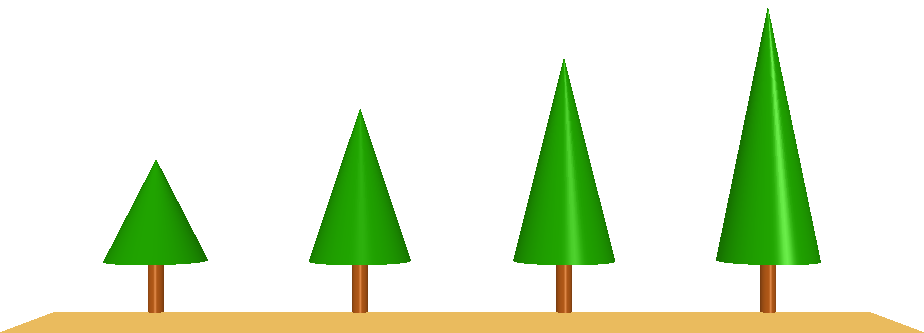
\includegraphics[width=5.5in]{\SMVfigdir/tree_line_objects}\\
 \end{tabular}
\end{center}
 \caption[A test showing trees drawn as Smokeview objects.]{A test
 showing trees drawn as Smokeview objects.  The tree canopy is
 colored green drawn as a cone,  the tree trunk is colored brown
 drawn as a cylinder.}
\label{figWUItrees}%
\end{figure}

\begin{figure}[bph]
\begin{center}
\begin{tabular}{cccc}
 
\includegraphics[width=1.5in]{\SMVfigdir/tree_test_state1}&
 
\includegraphics[width=1.5in]{\SMVfigdir/tree_test_state2}&
 
\includegraphics[width=1.5in]{\SMVfigdir/tree_test_state3}&
 
\includegraphics[width=1.5in]{\SMVfigdir/tree_test_state4}\\
 state 1&state 2&state 3&state 4
 \end{tabular}
\end{center}
 \caption[A test showing four states of smokeview tree objects.]
 {A test showing four states of the smokeview trunk and canopy objects.
 The  states are unburned trunk and canopy, burned trunk and canopy,
 burned trunk (canopy burned away), both canopy and trunk burned away.}
\label{figWUIstates}%
\end{figure}
\npage

Figure \ref{figWUIparts} shows an example of a tree drawn as particles and an isosurface.
Particle represent small units of fuel. Particle color represents
temperature.  As particles use up fuel they disappear. When many
trees are simulated, it is difficult to discern individual trees
when drawn as particles.  The second column of images in Fig. \ref{figWUIparts} shows an equivalent
view using an isosurface. The isosurface location is determined
from the boundary (between particle and non-particle regions in
the simulation) of the  particle cloud.
Figure \ref{figWUItreepart} show a particle file drawn using canopy objects.
The objects are colored according to the particle color as computed by FDS.


\begin{figure}[bph]
\begin{center}
\begin{tabular}{rcc}
\SI{0}{s}&\includegraphics[width=2.5in]{SCRIPT_FIGURES/pine_tree_part_000}&
\includegraphics[width=2.5in]{SCRIPT_FIGURES/pine_tree_partiso_000}\\
\SI{10}{s}&\includegraphics[width=2.5in]{SCRIPT_FIGURES/pine_tree_part_010}&
\includegraphics[width=2.5in]{SCRIPT_FIGURES/pine_tree_partiso_010}\\
\SI{20}{s}&\includegraphics[width=2.5in]{SCRIPT_FIGURES/pine_tree_part_020}&
\includegraphics[width=2.5in]{SCRIPT_FIGURES/pine_tree_partiso_020}\\
\SI{30}{s}&\includegraphics[width=2.5in]{SCRIPT_FIGURES/pine_tree_part_030}&
\includegraphics[width=2.5in]{SCRIPT_FIGURES/pine_tree_partiso_030}\\
 \end{tabular}
\end{center}
 \caption[A test showing trees drawn as particles and isosurfaces.]
 {A test showing trees drawn as particles and isosurfaces at \SI{0}{s}, \SI{10}{s},
 \SI{20}{s} and \SI{30}{s}.  Particle represent small units of fuel.
 Particle color represents temperature.  As particles use up fuel they disappear.}
\label{figWUIparts}%
\end{figure}

\begin{figure}[bph]
\begin{center}
\begin{tabular}{cc}
\includegraphics[width=3.5in]{SCRIPT_FIGURES/tree_test2_part_00}&
\includegraphics[width=3.5in]{SCRIPT_FIGURES/tree_test2_part_03}\\
\includegraphics[width=3.5in]{SCRIPT_FIGURES/tree_test2_part_06}&
\includegraphics[width=3.5in]{SCRIPT_FIGURES/tree_test2_part_09}\\
 \end{tabular}
\end{center}
 \caption[A test showing particles drawn as canopy objects.]
 {A test showing particles drawn as canopy objects
 at \SI{0}{s}, \SI{3}{s},
 \SI{6}{s} and \SI{9}{s}.  The canopy is colored according to temperature.}
\label{figWUItreepart}%
\end{figure}

\npage
